% Created 2022-03-31 Thu 01:57
% Intended LaTeX compiler: pdflatex
\documentclass{IEEEtran}
\usepackage[utf8]{inputenc}
\usepackage[T1]{fontenc}
\usepackage{graphicx}
\usepackage{longtable}
\usepackage{wrapfig}
\usepackage{rotating}
\usepackage[normalem]{ulem}
\usepackage{amsmath}
\usepackage{amssymb}
\usepackage{capt-of}
\usepackage{hyperref}
\usepackage[backend=biber, style=numeric]{biblatex}

\addbibresource{reference.bib}
\author{Anak Wannaphaschaiyong}
\date{\textit{<2022-03-03 Thu>}}
\title{Ensemble Approaches for Streaming Networking Classification}
\begin{document}

\maketitle

\section{Introduction}
\label{sec:orgb8220b8}
Often, real world problems involve entities and their relationship. This is best represented by graph data structures. In the case where graphs evolve overtimes, dynamic graph can be used to model them.

In the field of machine learning, dynamic graph modeling is still under explored, but its applications has been explored more recently in the past few years. Applications involve tasks such as graph protection, link prediction, entity/relation prediction, node clustering, node classification, and node attribute prediction (aka node regression), just to name a few \cite{kazemiRepresentationLearningDynamica}. Dynamic graph models are used to solve real world application involves traffic prediction \cite{yuanSurveyTrafficPrediction2021}, recommendation system \cite{kazemiRepresentationLearningDynamica}, knowledge graph completion \cite{cai2022temporal}, ecological network, distributed computing, interactions of economic agents, brain networks, \cite{holme2015modern}

Reinforcement learning was used to solve tasks such as graph protection problems on dynamic graph \cite{wijayanto2018learning,wijayanto2019effective}. For example, Meirom at el. \cite{meirom2021controlling} uses graph neural network to propagate information and reinforcement learning to rank highly infectious candidate. As of recently, during the Covid-19 pandemic, Kapoor et al. \cite{kapoor2020examining}  applies graph neural network on mobility data, which is represented as dynamic graph data, to predict state cases (represented as node value). The task to predict node's value is called node attribute prediction and also known as node regression task.
Dynamic graph is a vaguely used term. In general, dynamic graph is an ordered list of node and link events. These events include deletion and addition of nodes and edges after a interval of time. Dynamic graph has many (not perfectly) equivalent names with conflicting meaning as streaming graph and temporal graph. Embedding dynamic network surveys have been published to clarify terminology by purposing their own taxonomies \cite{barrosSurveyEmbeddingDynamic2021,kazemiRepresentationLearningDynamica,skardingFoundationsModelingDynamic2021}. We adopt taxonomy presented by Skarding et al. \cite{skardingFoundationsModelingDynamic2021} because it puts emphasis on taxonomy of dynamic graph neural network (DGNN), in particular, rather than deep learning on dynamic graph in general.
In static network, one must consider type of network relationship (e.g idealize network, proximity network.), scale of network (e.g. a node as a single entity, a node as a group of entities.), and network variation (link types e.g. homogeneous network, heterogenous network, multilayer network). Each mentioned factors encounters its own unique challenges. Importantly, these factors must be considered before model designing phase begins otherwise network based models cannot be expected to be compared fairly with other models. Moreover, it provide mental framework to guide designing process.

Dynamic graph extends static graph to include time variables which added time dimension to the problem. With time dimension to consider, models also must consider the following factor in addition to static network's factors mentioned previously: temporal granularity \cite{skardingFoundationsModelingDynamic2021}, temporal properties, dynamic behavior on graph, and n-dimension topological evolution \cite{holme2015modern,barrosSurveyEmbeddingDynamic2021}. Temporal granularity concerns time information that are kept in a graph which broken down to unweighted static graph (no time information is preserved), weighted static graph, discrete graph (stack of multiple weighted static graph), continuous graph (all time information is preserved) \cite{skardingFoundationsModelingDynamic2021}. Temporal properties concerns temporal features of an entity that compose a graph such as nodes, edges, and motifs. The temporal dimension can yield non-trivial temporal features such as interaction distribution (distribution of all edges overtime), interevent distribution (distribution of an edges/event over time), among others \cite{holme2012temporal,holme2015modern}. Interevent time distribution is the frequency distribution between the events. If the events are independent and drawn from a uniform distribution, then the inter-event time distribution will be exponential. However, empirical data set usually has fat-tailed, scale-free rather than uniform distribution. Coefficient of variation, bustiness, is used to characterized scale-free degree inter-event distribution. Dynamic behavior on graph concerns non-graph temporal features, such as communication behavior between nodes and substructure like motifs, and process on the network such as diffusion cascades. Lastly, n-dimension topological evolution involves structure evolution, features evolution, role evolution of nodes in a graph.

For static network, degree distribution is established itself as one of the most fundamental statistic. However, the argument does not hold true even for the simplest form of temporal network \cite{holme2015modern}. Simple temporal feature such as time of node and edges first appearance, time interval of node/edges presents from beginning to the end under some conditions are more important factor concerning nodes dynamic and evolution of graph structure.

Using data-driven approach, collected data usually contains too few data point to accurately measure temporal structure. Moreover, temporal structure, such as link burstiness, between node often has a fat-tailed distribution which is a problem when average over the value and most link occurs too little to be good representation of burstiness. Hence, we want to emphasize that quality of dataset that machine learning and deep learning models are trained on need to be improved by controlling quality over temporal properties of collected data. \cite{holme2015modern}

Another problem that unique to dynamic graph is representation. Holme et al. \cite{holme2012temporal} discuss that temporal properties depends on underlying dynamic graph representation, such as different network, aggregated network, time-varying network (a graph where edges are labeled based on time interval where they present in the graph), and multilayer network. For this reason, graph construction should be considered as an extremely important models design decision of data driven approaches such as deep learning. Deep learning models are directly trained on graph representation. Nonetheless, this topic doesn't get as much attention as it should. Furthermore, according to Holme et al. \cite{holme2015modern}, problem of representation of graph has been solved yet. There is no way to include all relevant dimension of dynamic graph into one complete dynamic graph representation. At the moment, which representation to choose depends on representation's accuracy and information one is willing to include or discard. That's it. Hence, one must chooses to represent dynamic graph in lossy and lossless ways. In addition to direct impact on the models of representation, illustrations are great to support discussion, without specifying assumption of the representation clearly, motivation of the purposed model and problem that the author solves can be misinterpreted or, even worse, misleading. For more information please refer to Holme et al. \cite{holme2015modern}

Dynamic graph representation can also be modified. This is done by adding synthetic edges. Synthetic edges can be added to dynamic graph representation which involves adding edges between nodes that has physical connection. Kapoor et al. \cite{kapoor2020examining} constructs graph as discrete graph and synthetic edges are added between the same nodes across multiple aggregated graph.
In general, performance between dynamic network based models are compared based on two main tasks link prediction and node classification. This is because these tasks are downstream task that can be tested on off-the-shelf approach. In static graph, link prediction task goal is to predict existence of pre-existence edges. On the other hand, according to Barros et al. \cite{barrosSurveyEmbeddingDynamic2021}, link prediction on dynamic graph task can be categorized into temporal link prediction and link completion. Similar to link prediction on static graph, link completion predicts existence of pre-existence edges at timestep \(t\). Temporal link prediction task, on the other hands, predict new edges. In this paper, we evaluate models on temporal link prediction tasks.

Dynamic node classification are less common compared to dynamic link prediction. This is because popular dataset for dynamic network tasks doesn't consider node labels. Commonly used dataset (within deep learning on dynamic graph domain) such as Reddit data provided node labels, but it is highly imbalance. Reddit data is used in the paper. In Dataset section, we will discuss the reproducible approach to create node labels for Reddit data.
In attempt to solve dynamic graph tasks, previous literature extends existing static network models. Gu et al. \cite{qu2020continuous} construct dynamic graph input into stack of weighted static graph by aggregating graph within fixed interval and feed the input to modified GCN model. More recently, models concerning continuous temporal granularity was purposed. TGAT was the first continuous DGNN to encode time by utilizing functional time embedding similar to time2vec. TGAT use information retrieval based attention which is parameterized by query, key, value --- first proposed by transformer \cite{vaswani2017attention}. TGN \cite{rossi2020temporal} adds memory module to TGAT. Our ensemble models is build on top of TGN.
So far, we have mentioned design aspects of dynamic graph models that are overlooked by community of deep learning on dynamic graph. In addition to that, relevant literature on the topics still uses simply train-test split to evaluate models performance. Dynamic graph is a sequential data and it is more appropriate to be evaluated with sliding window approach. Sliding window evaluation is a well known technique that is a gold standard for evaluating sequential data such as time series data. Furthermore, we found that models capacity directly depends on sliding window parameters such as window size, epoch per window etc. Therefore, without adopting sliding window evaluation as a standard to evaluate performance of dynamic network, one cannot create a fair environment to compare performance between dynamic network based models \cite{skarding2021benchmarking}. For this reason, we adopt window sliding window evaluation to evaluate temporal link prediction and dynamic node classification. The paper analyzes variations of ensemble approaches which can only be done when consider parameters from sliding window evaluation. Considering temporal factors mentioned above, the paper compare, analyze, establishes a generalized approach to implement ensemble models for dynamic graph models.
[What are brief results of the proposed design?] It is not yet clear to me what I should write for this.

\section{Related Work}
\label{sec:orge8a9f9d}
\subsection{Static Graph Modeling}
\label{sec:org7cf03ff}

Literature has tried to generalized convolution filter by generalized CNN grid filter for graph input. This only works for specific kind of graph that modified CNN grid is designed for. Another way to explore convolution filter is to convert graph from graph domain into frequency domain or Fourier domain. Filter in Fourier in domain is called spectral filter proposed by Defferard et al. \cite{defferrard2016convolutional} by using K-localized convolutional neural network on graph. Based on \cite{defferrard2016convolutional}, Kipf el at. \cite{kipf2016semi} purposed GCN where K is 1 and approximation of convolution filter is not learned by neural network rather than explicitly parameterize with Chebyshev approximation. GCN is one of the first GNN architecture that successfully applied as semi-supervised model. Downside of GCN is designed for transductive setting because graph Laplacian is known during the training. GraphSage \cite{hamilton2017inductive} solves the problem by using generalized neighbor information aggregation function (message passing framework), instead of diffuse information to neighbor with graph Laplacian. This also helps reduce over-fitting. Models using graph Laplacian or alike such as GCN is called spectral-based GNN while models that use neighbor aggregation function is called spatial-based GNN.

[discuss history of static GNN development after generalization of message passing.]

\subsection{Dynamic Graph}
\label{sec:org047224b}
\subsubsection{Taxonomies of Dynamic Graph}
\label{taxonomies of dynamic graph}
\begin{enumerate}
\item {\bfseries\sffamily TODO} I don't think ``dynamic over graph'' and ``dynamic on graph'' change this into something like ``node dynamic'', ``graph evolution''  which depends on 3 factors:
\label{sec:orgfc5edbe}
At the time of writing, multiple taxonomies of dynamic graph models has been proposed. In this related work section, we will discuss previous attempts to categorize dynamic graph models into groups. Before discussing previous attempt, one should understand types of dynamic behavior that can affect dynamic graph models. There are two types of dynamic behaviors which are referred to in referenced literature by different names, nonetheless, we will refer to the two types as ``dynamic behavior on graph'' and ``dynamic behavior over graph''. One can think of dynamic behavior on graph as communication between nodes that happens via edges. Dynamic  behavior over graph can be think of as changes of graph as a whole over time. Intuitively, ``dynamic behavior on graph'' concerns micro (node/edges) levels while ``dynamic behavior over graph'' concern macro level --- concern graph as a whole. An example to emphasize on the difference, given that there exist a group of individuals, Evolution of individuals (nodes) ``role'' depends on when and how they interact. At the macro level, a member of a group may leave and join. This behavior also depends on time interval that experiment considers.

Furthermore, design of models directly depend on dynamic behavior involved in dynamic graph. Hence, due to the factor mentioned above, it is very important to create an environment that is fair to make comparison between dynamic graph models. In addition to factor mentioned above, there are other factors that directly influence behavior on/over a graph including size of graph, node scale, et cetera, which beyond the scope of the paper. Empirical experiment has shown that combination of factors previously mentioned produces different temporal characteristic of dynamic graph either on/over the graph e.g. bustiness property \cite{holme2012temporal} among other.

Barros et al. \cite{barrosSurveyEmbeddingDynamic2021} categorized dynamic graph based on output embedding, model approaches, and dynamic behavior over graph. On the other than, Kazemi et al. \cite{kazemiRepresentationLearningDynamica} discuss in-depth mathematical formulation of encoder-decoder, one of many model approaches. The discussion also cover other types of models that are more specialized such as dynamic knowledge graph and spatio-temporal graph.

Skarding et al. \cite{skardingFoundationsModelingDynamic2021} takes interesting approach to categorized dynamic graph based on edges duration into interaction networks, temporal networks, evolving networks, and strictly evolving networks. Furthermore, the paper classifies dynamic network models into statical models, stochastic actor oretied models, and dynamic network representation learning model. In comparison, Skarding et al. \cite{skardingFoundationsModelingDynamic2021} and Kazemi et al. \cite{kazemiRepresentationLearningDynamica} provides two different ways to categorize dynamic graph models. In contrast to Kazemi et al, Skarding et al. focus mainly on taxonomies of dynamic graph neural network including pseudo-dynamic model, edge-weighted model, discrete model, continuous models.

Note that meaning of temporal networks is ambiguous outside of skarding et al's paper \cite{skardingFoundationsModelingDynamic2021} context. In ``Temporal Network'' paper, Holme et al. \cite{holme2012temporal} introduce ``time-respecting'' path as a property of temporal network. Graph with time-respect path contains edges whose weight value represents time when edges forms. We will adopt taxonomy presented in \cite{skardingFoundationsModelingDynamic2021} because including adopting temporal network definition. This is unambiguous because time-respecting path has not explored at all in the machine learning at the time of writing. Furthermore, all types of dynamic graph can be represented as a form of multilayer graph. \cite{kivela2014multilayer}
\end{enumerate}
\subsubsection{Dynamic Graph Modeling}
\label{sec:org0ed4045}
Before designing dynamic graph models, one must consider construction of dynamic graph input based on dataset. Then, models can be designed on top of constructed input. Dynamic graph construction is out of scope of this paper, but it is important to emphasize that model architecture is heavily dependent on input. Example of input graph construction are aggregated graph (edge-weighted graph \cite{qu2020continuous}), synthetic link between static graph \cite{kapoor2020examining}, and different graph. When designing dynamic graph models, one must consider node dynamic, link duration, and temporal granularity. Node dynamic concerns presents of nodes. Link duration concerns presents of edges, and temporal granularity concern either discrete or continuous occurrence of events \cite{kazemiRepresentationLearningDynamica}.

History of deep learning solution of dynamic graph models can be traced back to 2016. At the time, literature explored methods of aggregating information on graph from node neighbor with varying weight, such as using tree like structure for NLP tasks and grid like structure. Furthermore, RNN had been used to learn temporal features while structure features are learned by CNN, GNN, or random walk. This can be done either by simply stacking temporal layer to structure layer or integrate temporal and structure components in to one layer \cite{seo2018structured}. Note that 2016 is around the peak of RNN hype. Around the same time, research effort was put toward the development of convolution filters. We discuss related work on this topic in Static Graph Modeling section. Later, Xu et al. \cite{xu2019generative} purposed G-GCN. The models disregard time and take into consideration only topology changes. This is done by extending variational Graph Autoencoder (VGAE) \cite{kipf2016variational} to predict unseen node.

In particular, according to dynamic graph modeling taxonomy \cite{kazemiRepresentationLearningDynamica}, this paper concerns continuous dynamic graph neural network (continuous DGNN). Continuous DGNN update information for every time an event (edge instance) occurs. Furthermore, these type of model can use temporal difference, time invertal between event, as input parameter. Neural network component can be used to approximate point process parameters. This approach is called temporal point process based model (TPP). On the other hand, neural network can be used to encode temporal pattern by learning representation of time embedding vector. TGN falls into this category.
\subsection{Representation of temporal network.}
\label{sec:org321f5d7}
lossless representation and lossly representation.
\subsection{Sliding Window Evaluation}
\label{sec:orgd515e3a}
\subsubsection{{\bfseries\sffamily TODO} Sliding window approaches turn any time series dataset into a supervised learning problem. Given that an instance in a dataset is an event with timestamp, train-test-split are a kind of sliding window where you only have 1 window to train to predict the future. Mathematically, consider dynamic networks observed at discrete time steps, \(1,2,...,T\). For each \(t = 1,...,T\), one trains model on window \(w_{t}\) where \(t=1,2,...,T-1\) to predict score of \(w_{\hat t}\) where \(\hat t=2,3,...,T\), respectively. Because temporal properties of time window, \(w\), depends on window size, \(ws\), and interval of time, \(\Delta t\), evaluating performance based on sliding window approach show model's performance under various temporal condition, such as temporal frequency, seasonality, cycles (business cycles, economy cycle, war, etc), serial correlation, hence, comparison between models are not fair without considering appropriate sliding window parameters.}
\label{sec:org4ebeb57}

Sliding window is specially important in dynamic based graph when applying ensemble models on top of dynamic graph models, as we will show later, overall performance depends on size of window, number of epoch per window, number of windows, number of batch per window, number of window, and time budget.

Furthermore, sequence of windows allows one to apply a higher level of abstraction over sequence of events which may influence models design. In this case, sliding window evaluation must be applied to all the models involve to create a fair comparison.

In the time of writing, dynamic graph model literature still uses simple train-val-test split as a model evaluation standards. We provide examples of well accepted paper to make a point. Tian et al. \cite{tian2021self} use 70-15-15 split to evaluate self-supervised learning on strictly evolving graph and compare with models. Performance of models are evaluated based on two tasks: link prediction and node classification. The comparison is limited to static graph models, and dynamic random walk. Details to extend static graph models to dynamic graphs are not discussed. Similarly, using the same dataset, Rossi et al. \cite{rossi2020temporal} also use 70-15-15 splits. Rossi et al. compare its own, temporal graph neural network (TGN) to one other dynamic graph, DyRep. The comparison is acceptable because same dataset is used in the experiment. Dataset used in mentioned papers are collected as undirected interaction network.

It is very important to understand that how models receive data --- stream data, one instance at a time, or in batch --- implies underlying graph type. This is because it implies existence duration of nodes and edges which is used to classify dynamic graph based on taxonomies proposed by Skarding et al. \cite{skardingFoundationsModelingDynamic2021}. For detail about taxonomies of dynamic graph can be found in \ref{taxonomies of dynamic graph} section.

To the best of my knowledge, Skarding et al. wrote ``BENCHMARKING GRAPH NEURAL NETWORKS ON DYNAMIC LINK PREDICTION'' \cite{skarding2021benchmarking} which is the only paper to compare dynamic network based models using sliding window evaluation. Directed and undirected interaction network is used. Interaction network can be easily aggregated to form ``graph snapshot.'' Hence, using interaction network, one can pass in continuous network to continuous model and discrete network to discrete models.

Performance of each model varies across metric score. Hence, the paper concludes that optimizing the hyperparamters is essential for obtaining a representative score. This conclusion applies for both static and dynamic graph models. Furthermore, Skarding et al. observes that using window of size 5 or 10 consistently produce best results particularly among discrete models.
\section{Approaches}
\label{sec:org0feaf0a}
\begin{table}[htbp]
\caption{\label{parameters}Parameters symbols and descriptions}
\centering
\begin{tabular}{lll}
\hline
\hline
 & parameters & description\\
\hline
window parameters & \(w_i\) & i-th window\\
 & \(ws\) & window size\\
 & \(\vert w \vert\) & number of window used during training\\
 & \(bs\) & batch size for a given window where \(bs < ws\)\\
temporal parameters & \(stride\) & window stride\\
 & \(pred\_next_{n}\) & predict instances that are in window that is n window away.\\
 & \(keep\_last\_n\) & number of window to keep as window slides forward\\
 & \(total\_training_windows\) & total number of instances to be trained for\\
ensemble parameters & \(E_i\) & i-th model in ensemble\\
 & \(\vert E \vert\) & number of models used in ensemble\\
 & \(train\_w_{i}\) & i-th window is the first window to begin training\\
granularity parameters & \(PW\) & granularity of prediction. Prediction length during training\\
\end{tabular}
\end{table}

\begin{figure}[htbp]
\centering
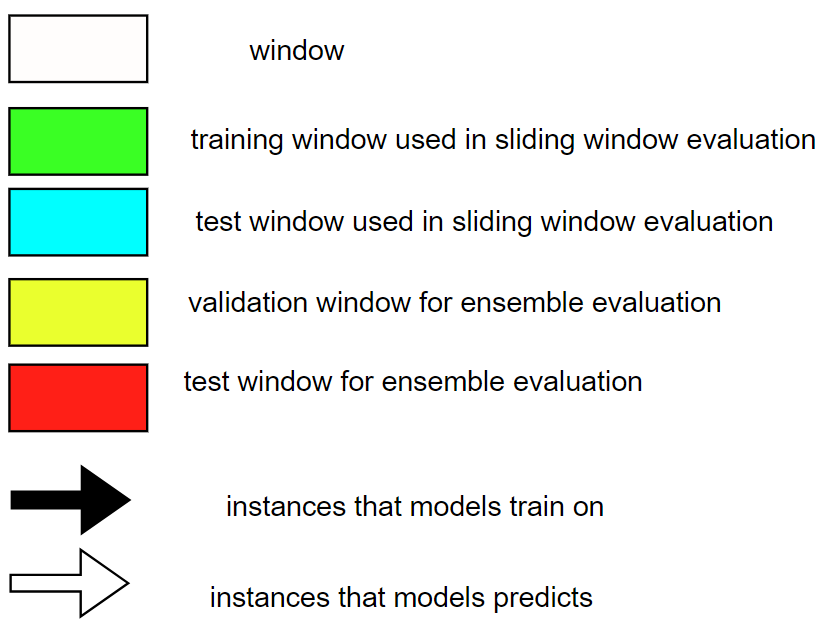
\includegraphics[width=.9\linewidth]{./images/screenshot_20220321_130824.png}
\caption{\label{symbols}symbols}
\end{figure}

\begin{figure}[htbp]
\centering
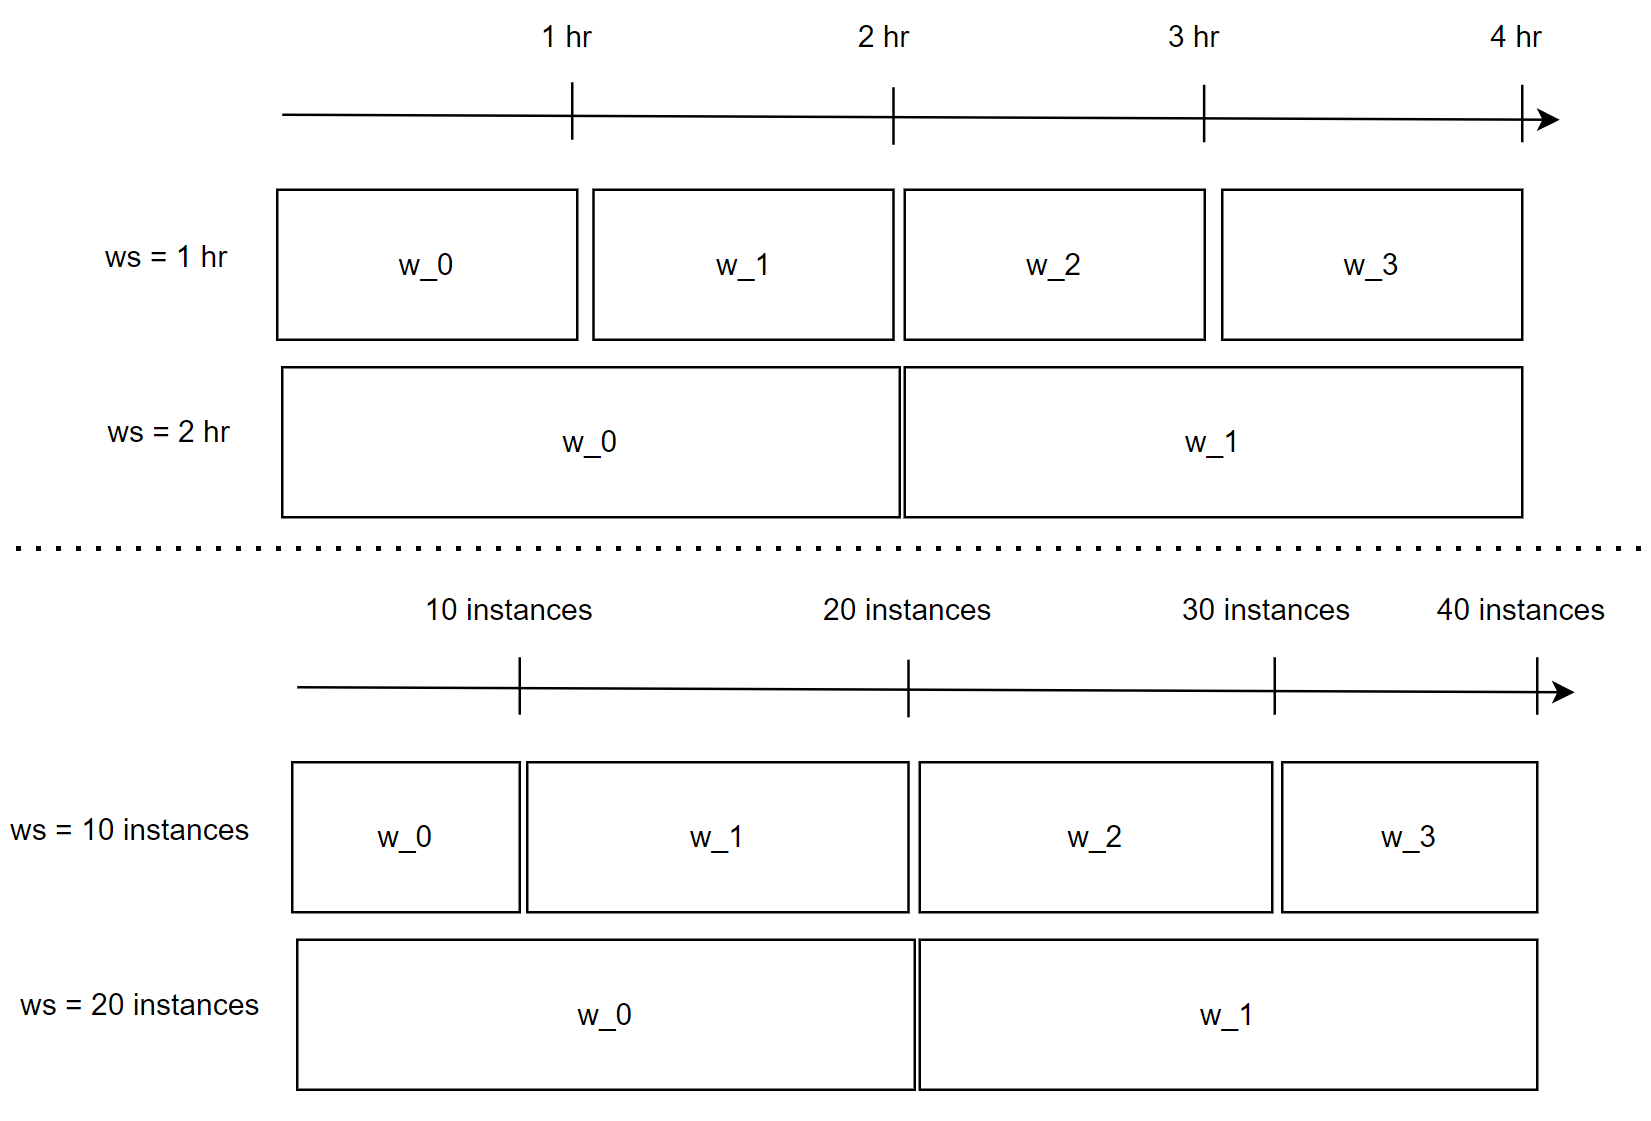
\includegraphics[width=.9\linewidth]{./images/screenshot_20220321_110302.png}
\caption{\label{window_parameters}window parameters}
\end{figure}

\begin{figure}[htbp]
\centering
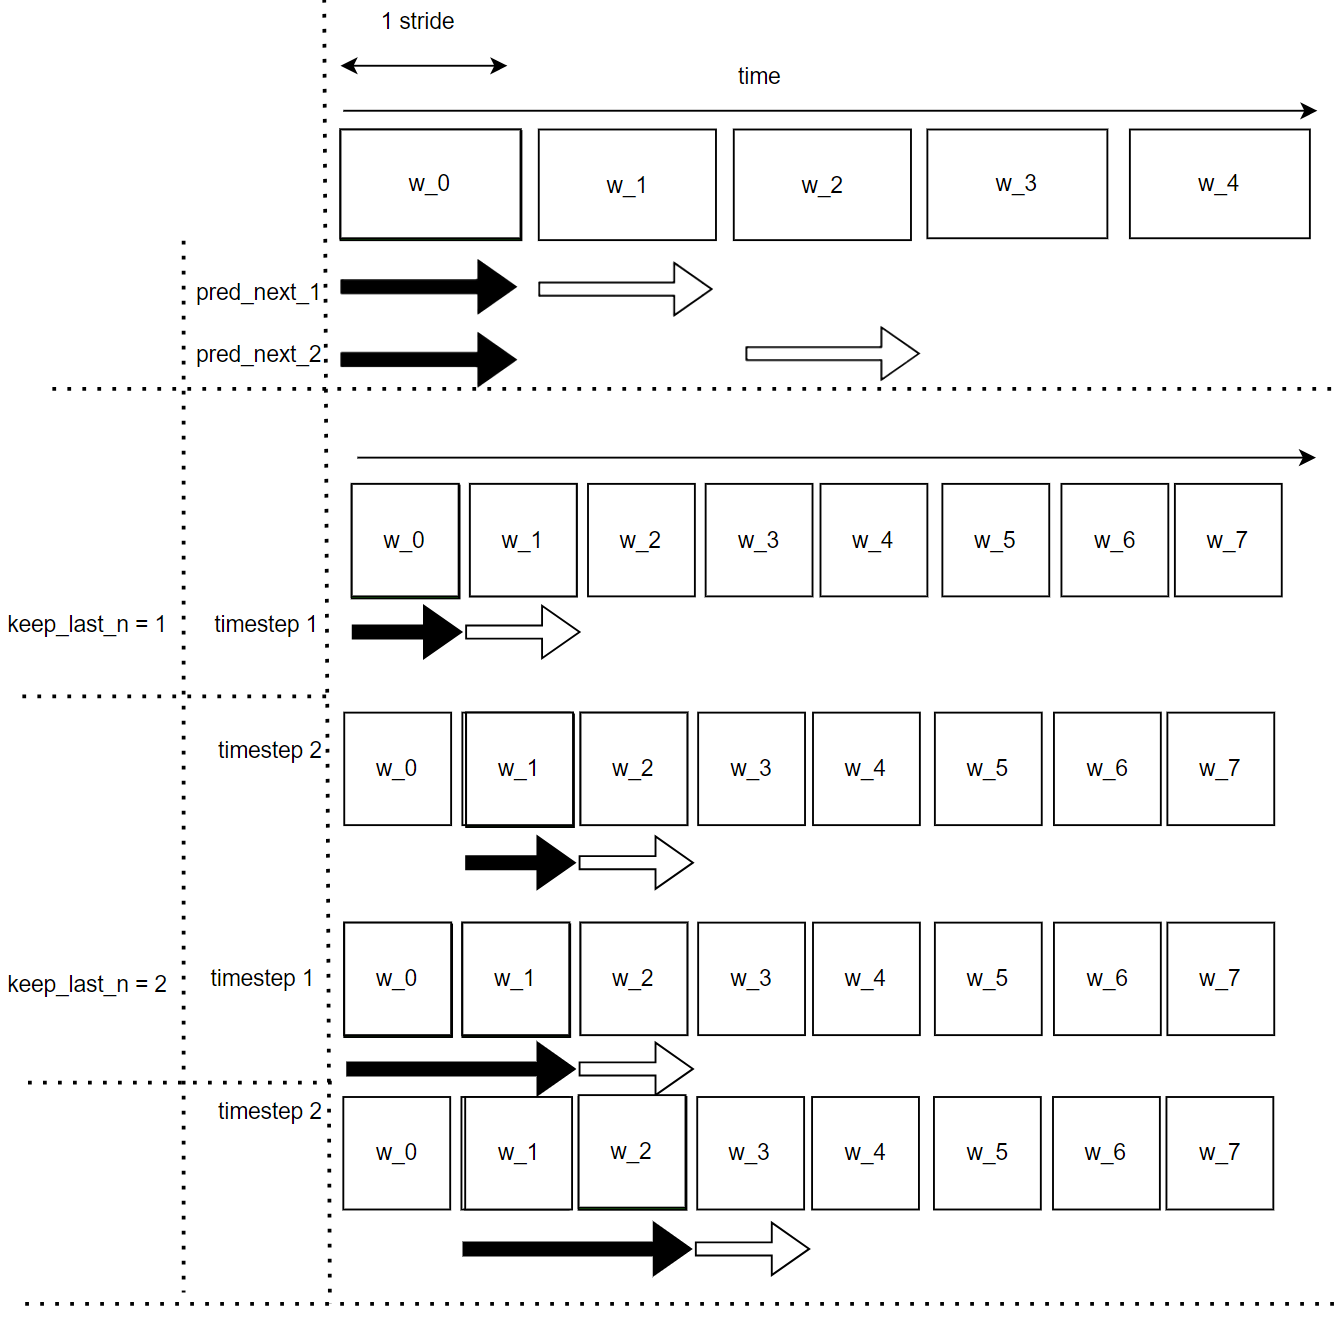
\includegraphics[width=.9\linewidth]{./images/screenshot_20220321_130701.png}
\caption{\label{temporal_parameters}temporal parameters}
\end{figure}

\begin{figure}[htbp]
\centering
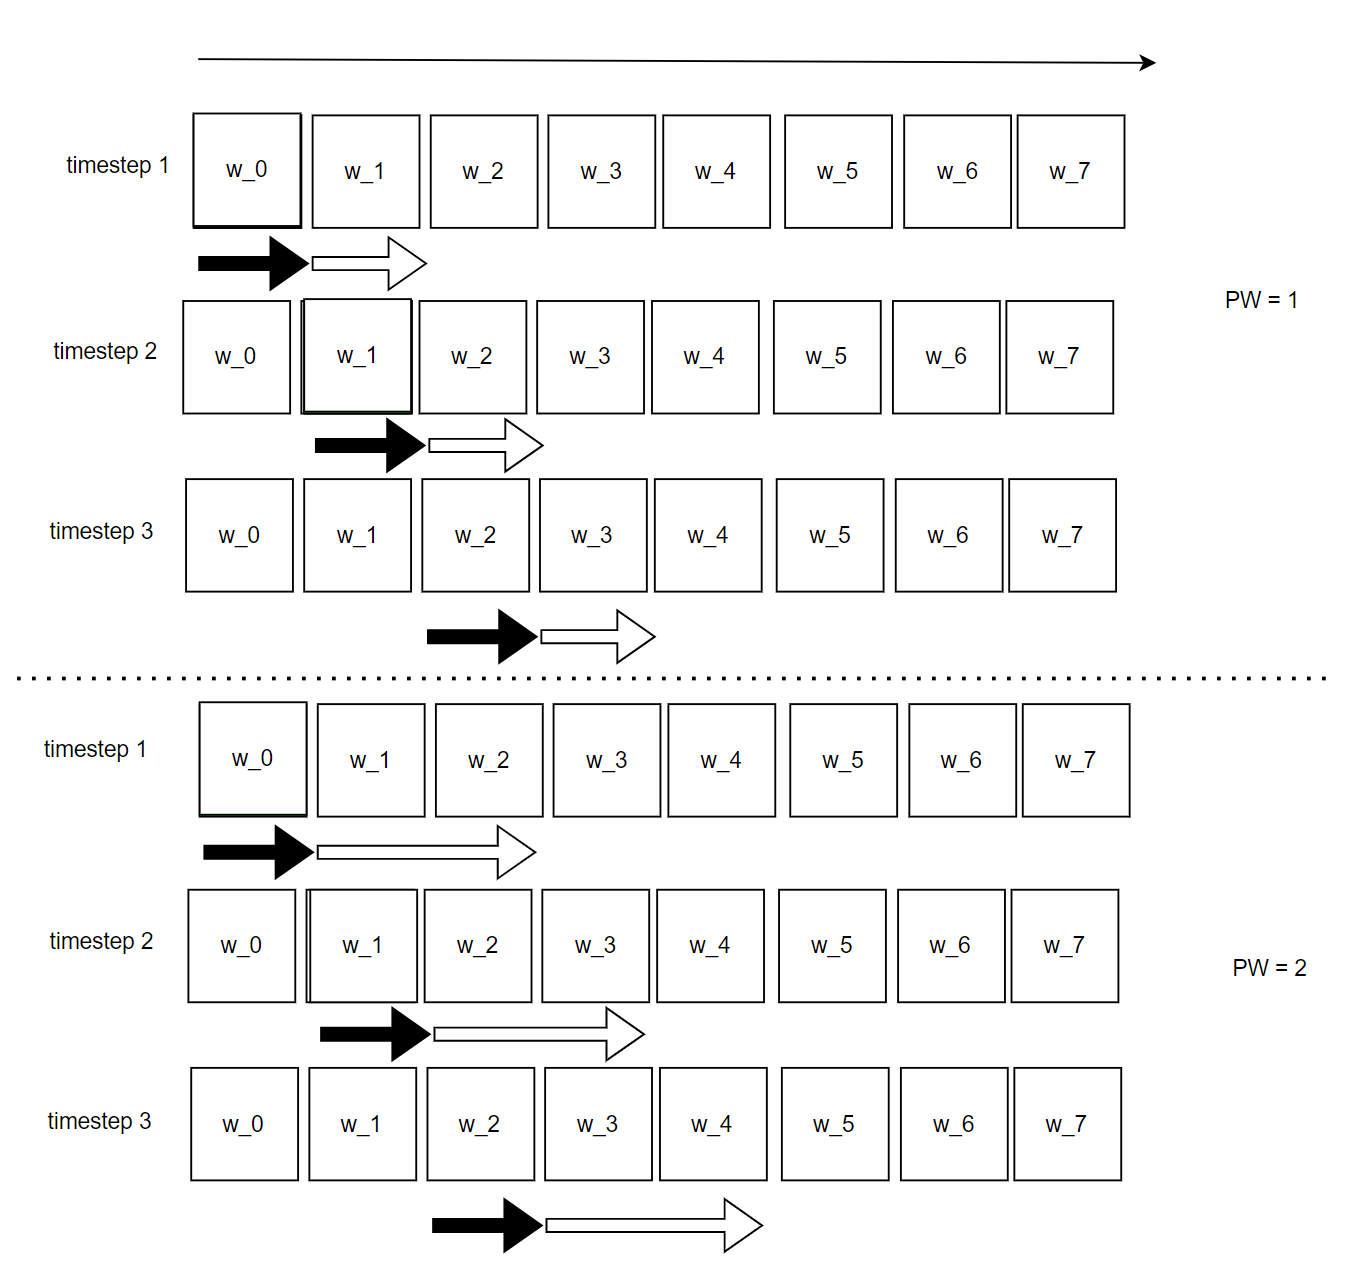
\includegraphics[width=.9\linewidth]{./images/screenshot_20220321_130720.png}
\caption{\label{granularity_parameters}granularity parameters}
\end{figure}


In sliding window evaluation setting, one needs to make sure proposed model and benchmark model is being tested as fair as possible. Furthermore, to extract the most benefit from ensemble models, participated models should provide diverse predictive information. Table \ref{parameters} provides list of parameters that must be considered to maximize diversity of predictive information in ensemble models.

According to Table \ref{parameters}, we categorize parameters of sliding window evaluation into four categories: windows parameters, temporal parameters, ensemble parameters, and granularity parameters.
Window parameters and ensemble parameters are self-explanatory, but granularity parameters and temporal parameters need clarification.
Granularity is determined by prediction length during training. This parameter is important because it tells the model to minimize its mistake for certain time interval. In the other word, a model whose prediction performance is optimized over 10 days will be different to model whose performance is optimized over one day. Larger model that is trained on larger granularity ignores short term stochasticity of temporal dependencies. Illustration of window parameters, temporal parameters, granularity parameters groups are provided in Figure \ref{window_parameters}, \ref{temporal_parameters}, and \ref{granularity_parameters}. Symbols used in figures followed Figure \ref{symbols}.

It is important to note that temporal parameters can be applied ``during ensemble formation'' and ``in-between ensemble formation.'' During ensemble formation referring to the modeling step where, given a fix set of training length, N number of individuals are trained before voting predictive score to finalize an ensemble performance. In contrast, in-between ensemble formation occurs after ensemble performance of the previous timestep is finalized and set of training instance is adjusted before it will be used to train an ensemble model of the next time step.

\begin{figure}[htbp]
\centering
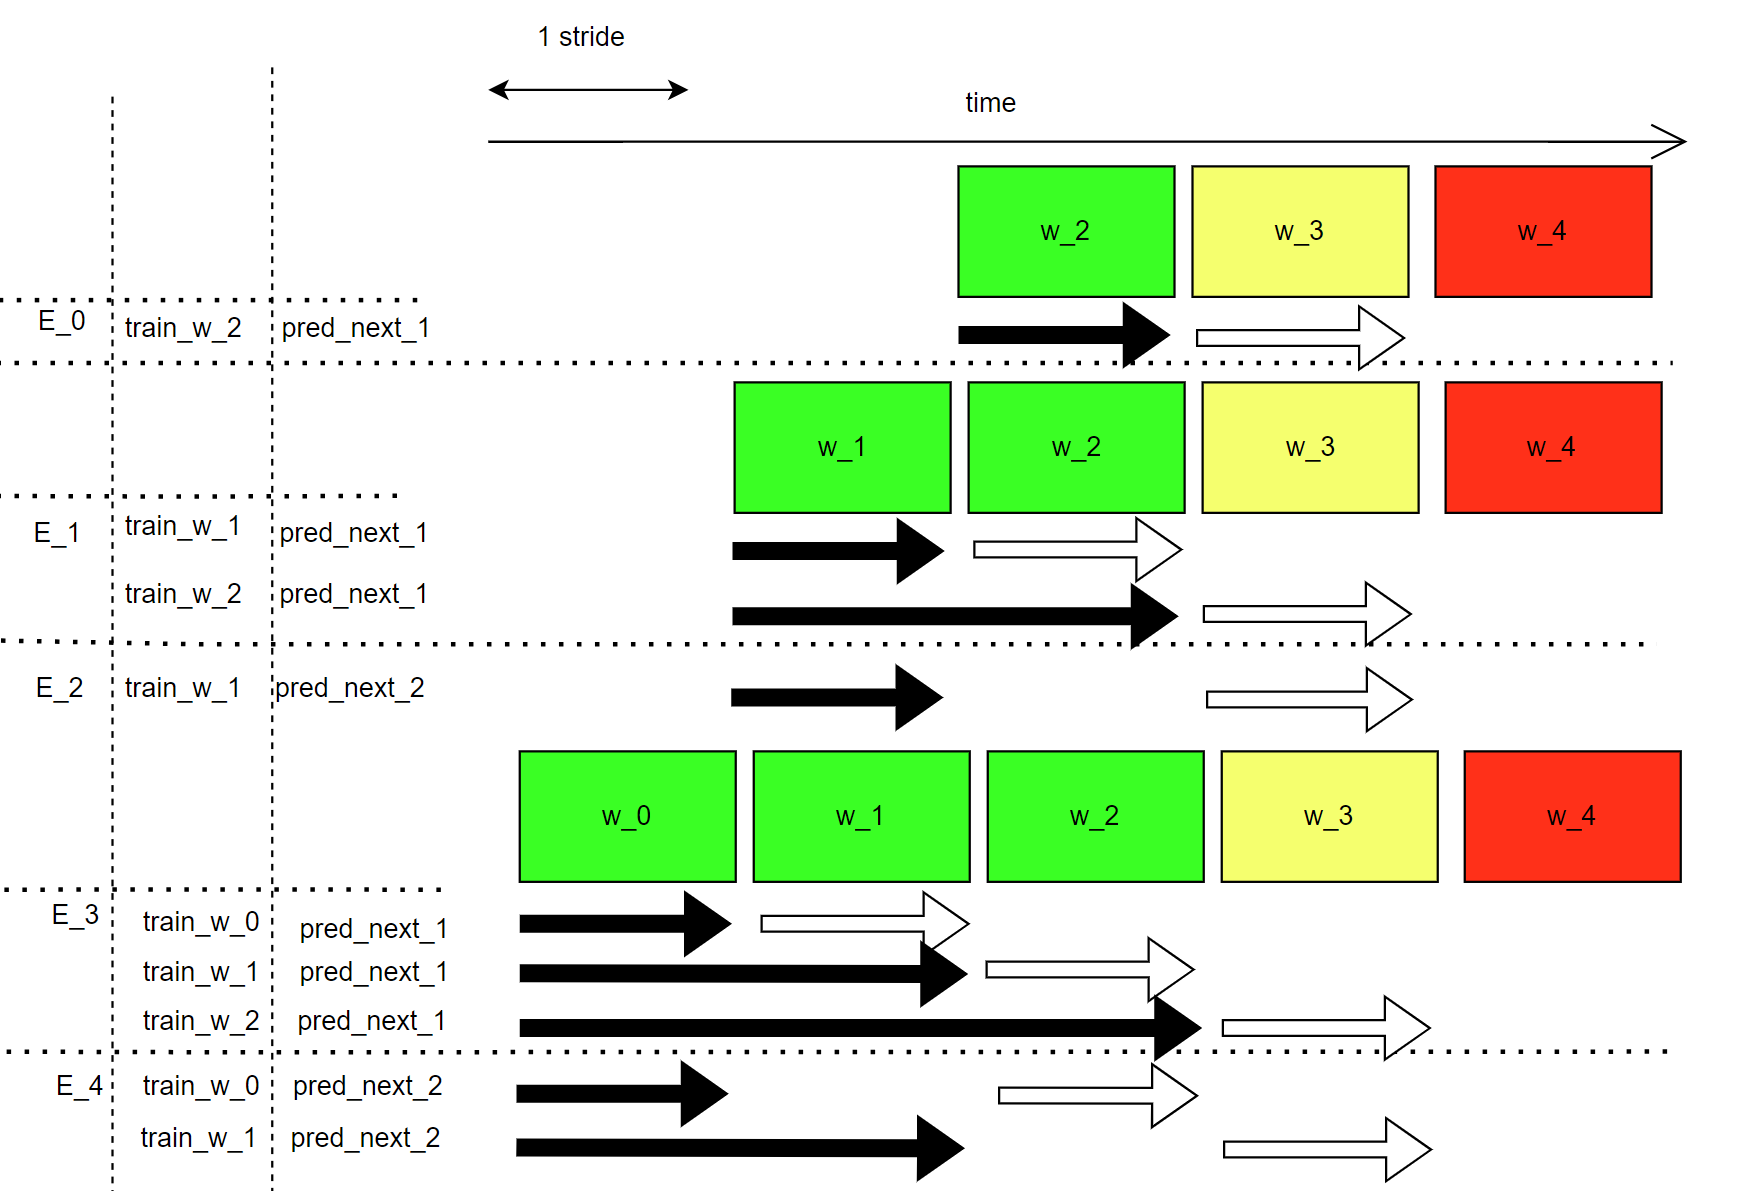
\includegraphics[width=.9\linewidth]{./images/screenshot_20220321_124235.png}
\caption{\label{ensemble_variation_1}ensemble variation 1}
\end{figure}

\begin{figure}[htbp]
\centering
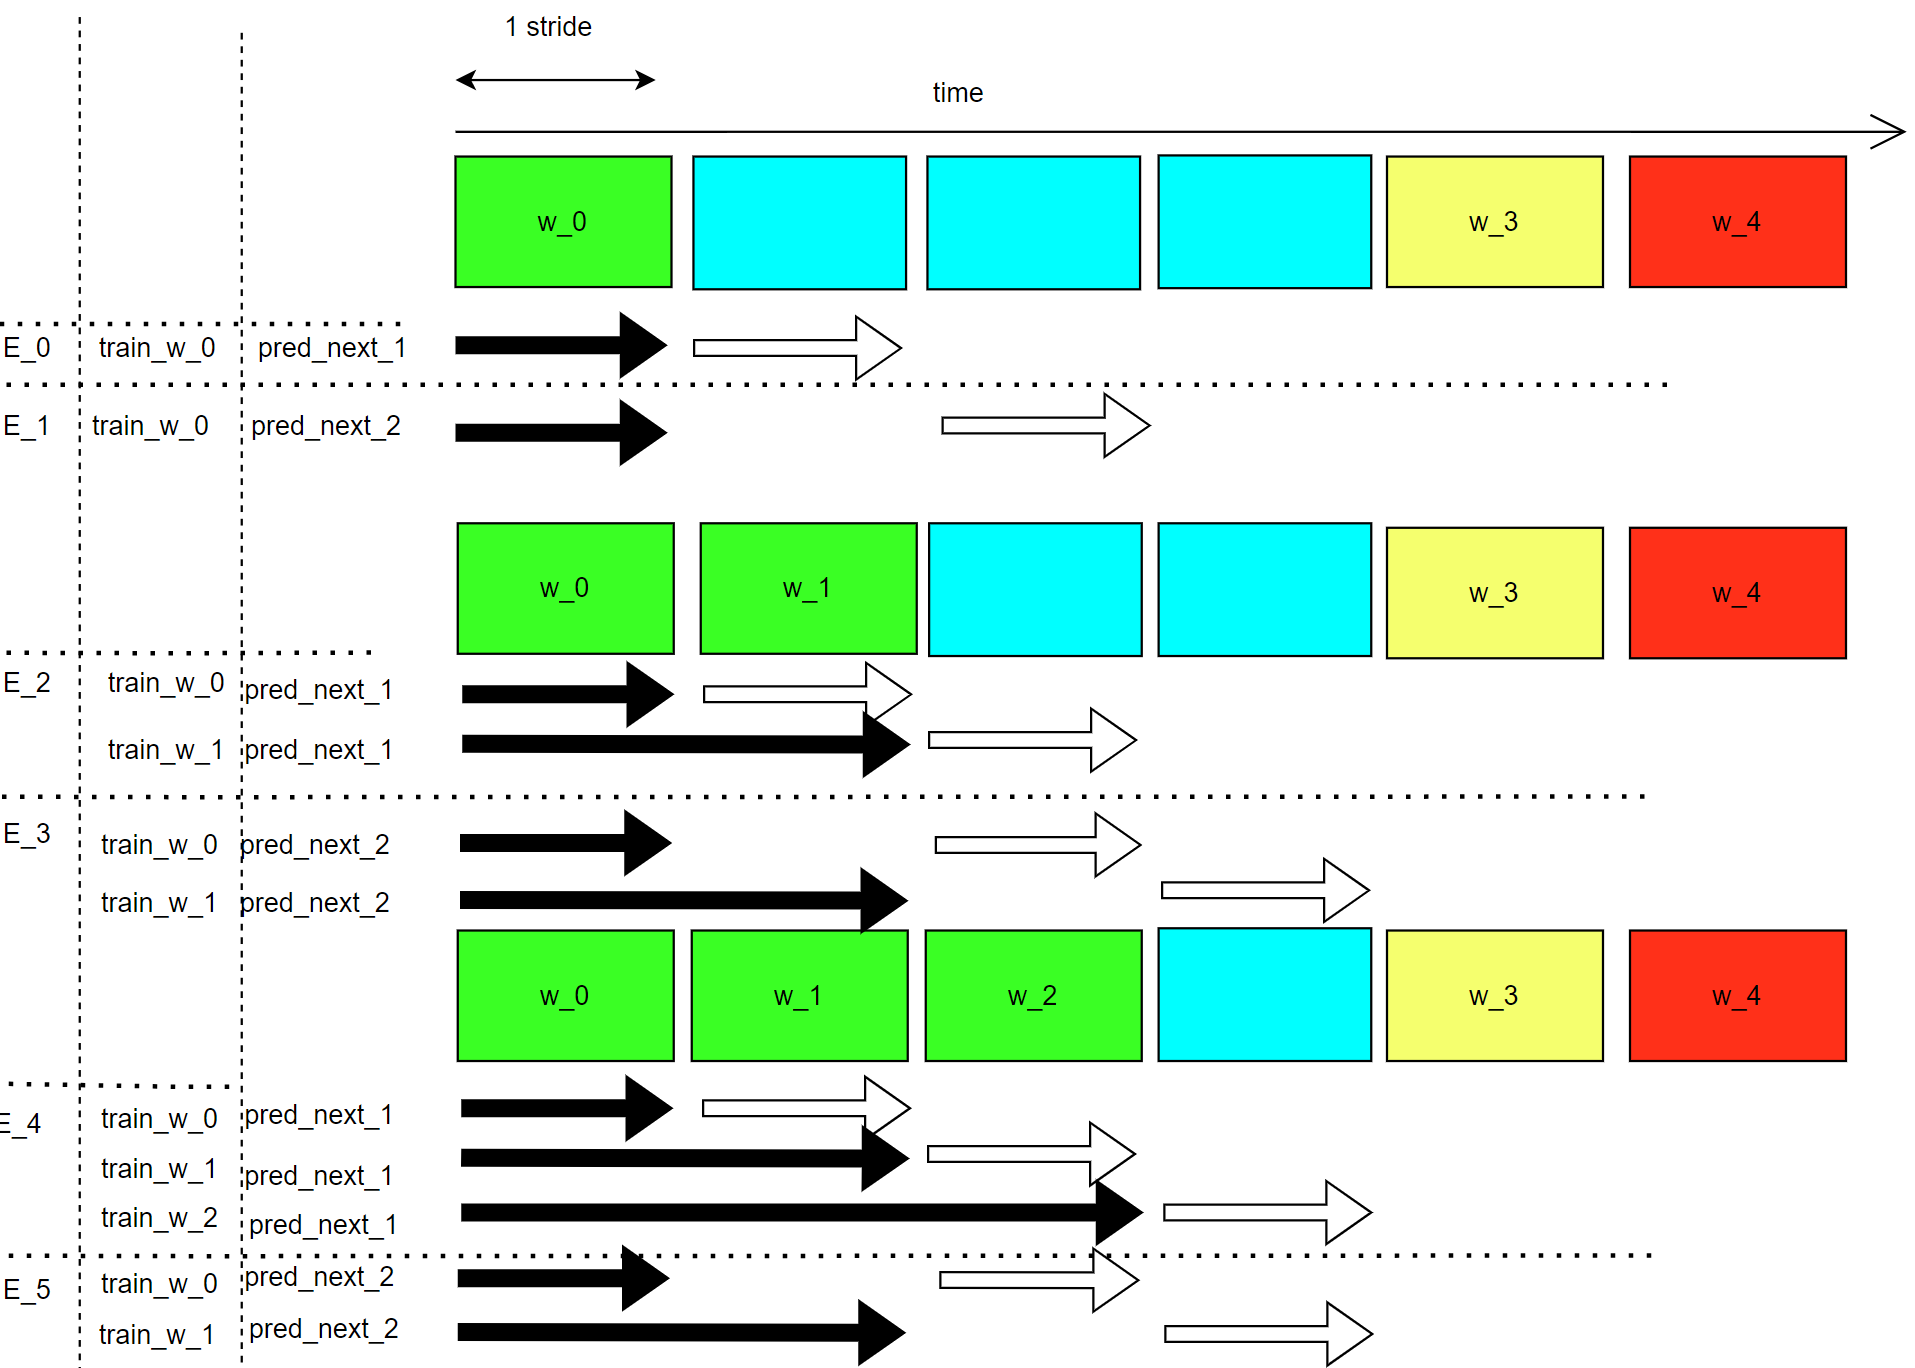
\includegraphics[width=.9\linewidth]{./images/screenshot_20220321_124707.png}
\caption{\label{ensemble_variation_2}ensemble variation 2}
\end{figure}

Using sliding window evaluation approach, there are a lot of combination of parameters that can effect model's predictive information. For this reason, one may consider using time budget to reduce size of solution space.
\section{Dataset}
\label{sec:orgf49acdd}
\textbf{Reddit dataset}: Reddit dataset are a bipartite network of interaction network involving two groups of nodes: Reddit threads and users. Row of the dataset is a tuple of including user-id, thread-id, timestamp, whether user is banned after this event, and pre-compute embedding score with 172 dimensions. There are 672448 instances of interaction (aka edges) which is collected in one month time interval with total 11,000 nodes. Property of Reddit dataset is shown in Table \ref{Datasets}.

\begin{table}[htbp]
\caption{\label{Datasets}Datasets}
\centering
\begin{tabular}{ll}
\hline
\hline
 & Reddit\\
\hline
\# Nodes & 11,000\\
\# Edges & 672,447\\
\# Edges Features & 172\\
Timestapn & 1 month\\
positive label percentages & 0.05 \%\\
\end{tabular}
\end{table}
\section{Results}
\label{sec:org136d33b}
\printbibliography
\end{document}
